%%%%%%%%%%%%%%%%%%%%%%%%%%%%%%
%%                                                     %%
%%   LaTeX template voor P&O: Computerwetenschappen.   %%
%%                                                     %%
%%   Schrijfopdracht 1                                 %%
%%                                                     %%
%%   7 oktober 2013                                    %%
%%   Versie 1.1                                        %%
%%                                                     %%
%%%%%%%%%%%%%%%%%%%%%%%%%%%%%%

\documentclass{peno-opdracht1}
\usepackage{comment}
\usepackage{pdfpages}
\usepackage{titlesec}
\usepackage{textcomp}
\usepackage{sidecap}
\usepackage{caption}
\usepackage{scrextend}
\titleformat{\section}
{\normalfont\fontsize{12}{15}\bfseries}{\thesection}{1em}{}

\team{Zilver} % teamkleur

\begin{document}

\maketitle

\noindent
	Ons team bestaat uit Bram Vandendriessche, Matthias Van der Heyden, Jef Versyck, Vincent Vliegen, Arne Vlietinck en Laura Vranken. Bram werd aangeduid als CEO en Arne zal de taak van CAO op zich nemen. \\
	Om op een effici\"ente manier het geheel te kunnen realiseren, wordt het team in twee verdeeld. De ene groep (Bram, Jef en Arne) buigt zich over het virtual testbed. Het andere team  (Matthias, Vincent en Laura) zorgt voor de drone autopilot.\\
	Een gedetailleerde planning kan teruggevonden worden in appendix \ref{App:Planning}.

\section{API keuze}
Als API voor het genereren van 3D-beelden selecteerden we drie kandidaten: Blender, JMonkeyEngine en OpenGL.\\
Blender heeft als voordeel dat voorwerpen gemakkelijk aangemaakt kunnen worden door de gebruiksvriendelijke interface. Blender gebruikt echter Python. Hierdoor wordt er een extra moeilijk-heid gecre\"eerd, namelijk de communicatie tussen Java en Python. Blender zou dan vanuit Java moeten worden gestart, wat in een omslachtig proces resulteert. Vooral omwille van deze laatste eigenschap zal er geen gebruik gemaakt worden van Blender. \\
JMonkeyEngine is gebruiksvriendelijker dan OpenGL, maar door gebrek aan uitgebreide communities wordt er niet voor geopteerd.\\
Onze keuze gaat uit naar OpenGL ondanks het ontbreken van een grafische interface. Dit nadeel kan wel gedeeltelijk omzeild worden door figuren te importeren vanuit Blender. OpenGL is reeds bruikbaar in Java en heeft bij problemen meer documentatie dan JMonkey.

\section{Autopilot}
De autopilot van de drone moet zijn positie ten opzichte van het doel kunnen bepalen aan de hand van twee ontvangen camerabeelden. Eerst wordt de diepte bepaald op basis van de brandpuntsafstand, de afstand tussen de zichtbare rode bol op het frame en het middelpunt van het frame (in pixels) en de afstand tussen de camera\textquotesingle s (in meter).\footnote{NASA tech briefs. (2012). A Guide to Stereovision and 3D Imaging. Geraadpleegd op 5 oktober 2016 via http://www.techbriefs.com/component/content/article/14925.\label{refnote}} Zie appendix \ref{App:Afstand}. \\
Om te vliegen, ori\"enteren we eerst de drone naar het doel. Hiervoor moeten opeenvolgend de rotaties (pitch, roll en yaw) onder een bepaalde hoek uitgevoerd worden. Vervolgens wordt naar het doel toe gevlogen via een combinatie van thrust en pitch.
Om te kunnen controleren of de drone nog in de juiste richting vliegt, worden de berekeningen na iedere draai of na een bepaalde vliegafstand opnieuw uitgevoerd.
Als pixel waarop de berekeningen gebaseerd worden, kiezen we diegene die het zwaartepunt van de gedetecteerde vorm weerspiegelt. Dit zwaartepunt bepalen we door de co\"ordinaten van alle rode pixels op te slaan en hieruit de gemiddelde x- en y-co\"ordinaat te berekenen.

\section{GUI}
De GUI zal gezamenlijk gemaakt worden, zodanig dat de vereisten van beide subgroepen erin verwerkt kunnen worden. \\

\newpage
\appendix
\section{Gantt chart} \label{App:Planning}

\begin{figure}[h!]
	\begin{center}
		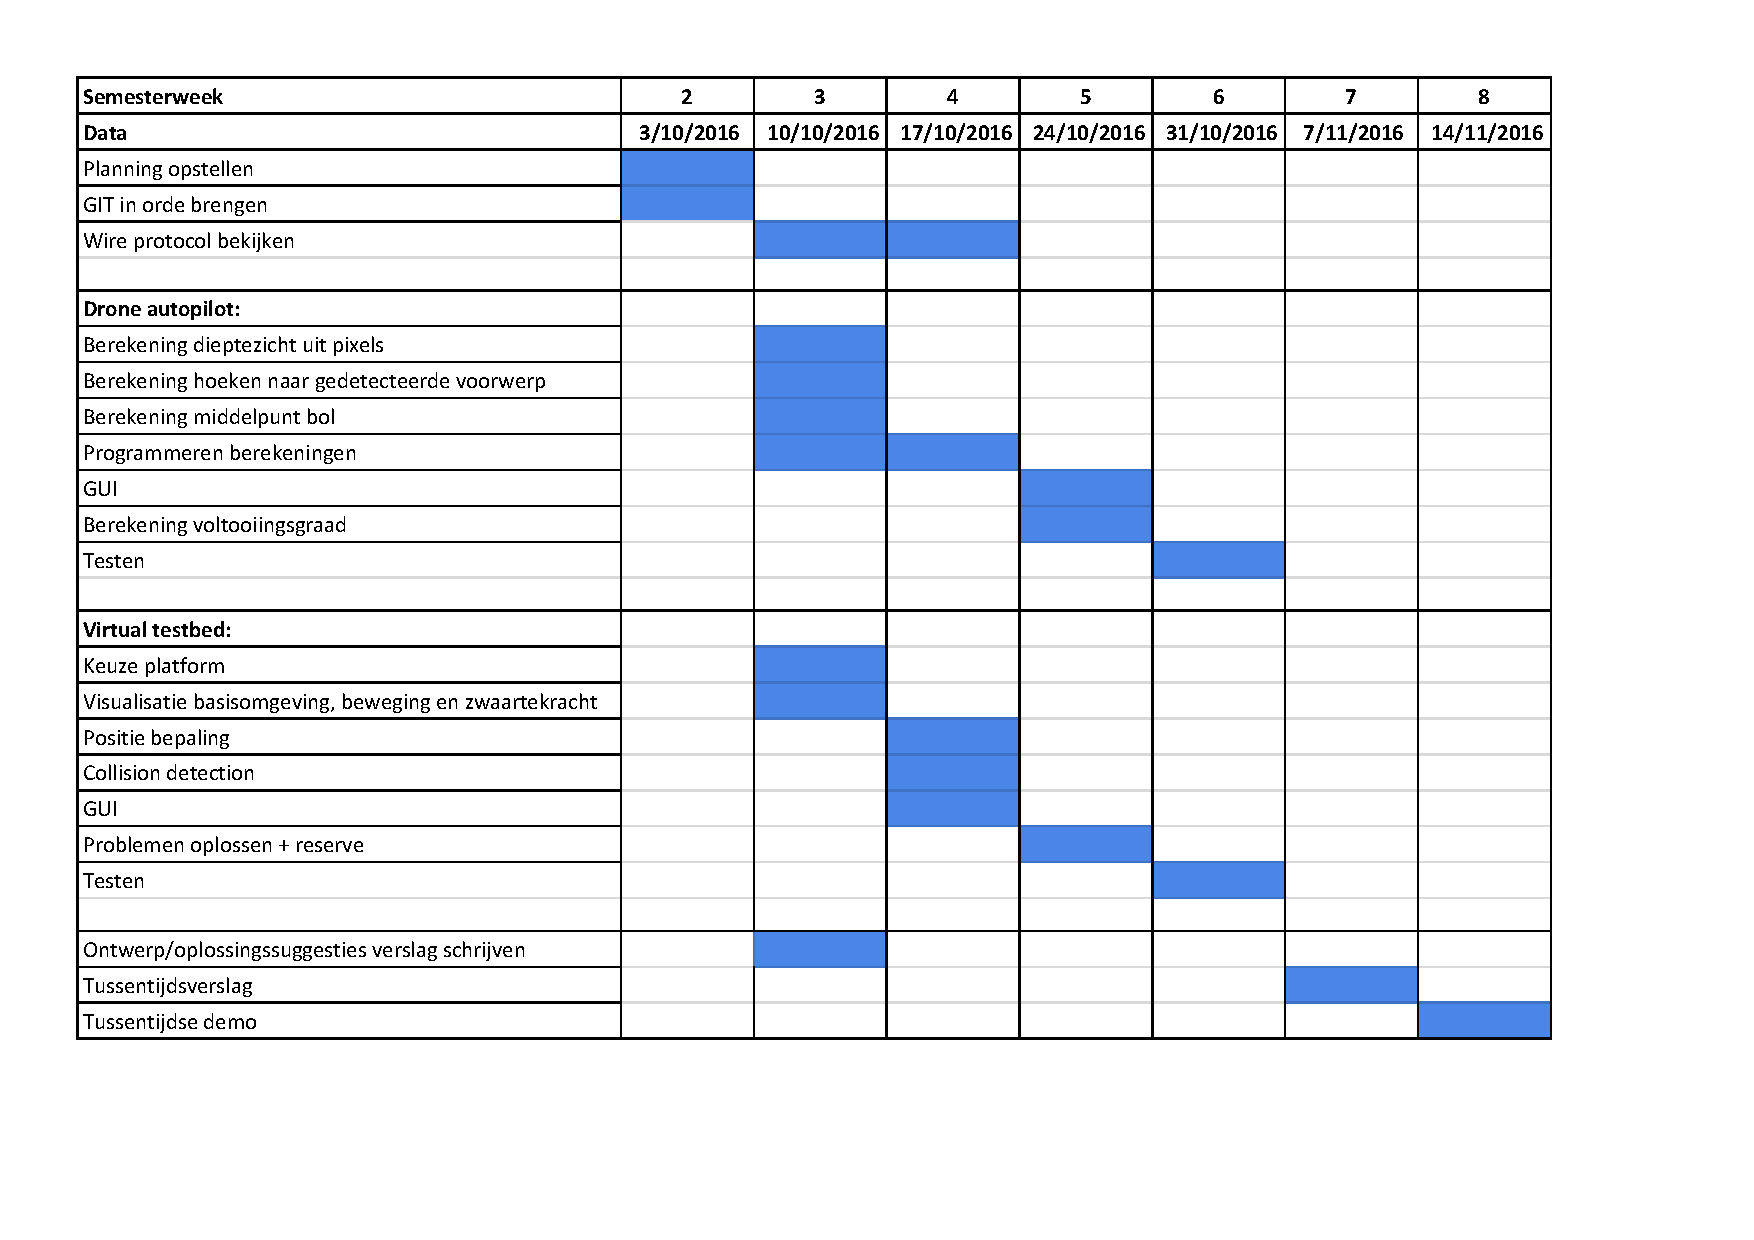
\includegraphics[scale=0.55]{Planning.pdf}
	\end{center}
\end{figure}

\section{Diepte-berekening} \label{App:Afstand}

\begin{figure}[h!]
	\begin{center}
		
		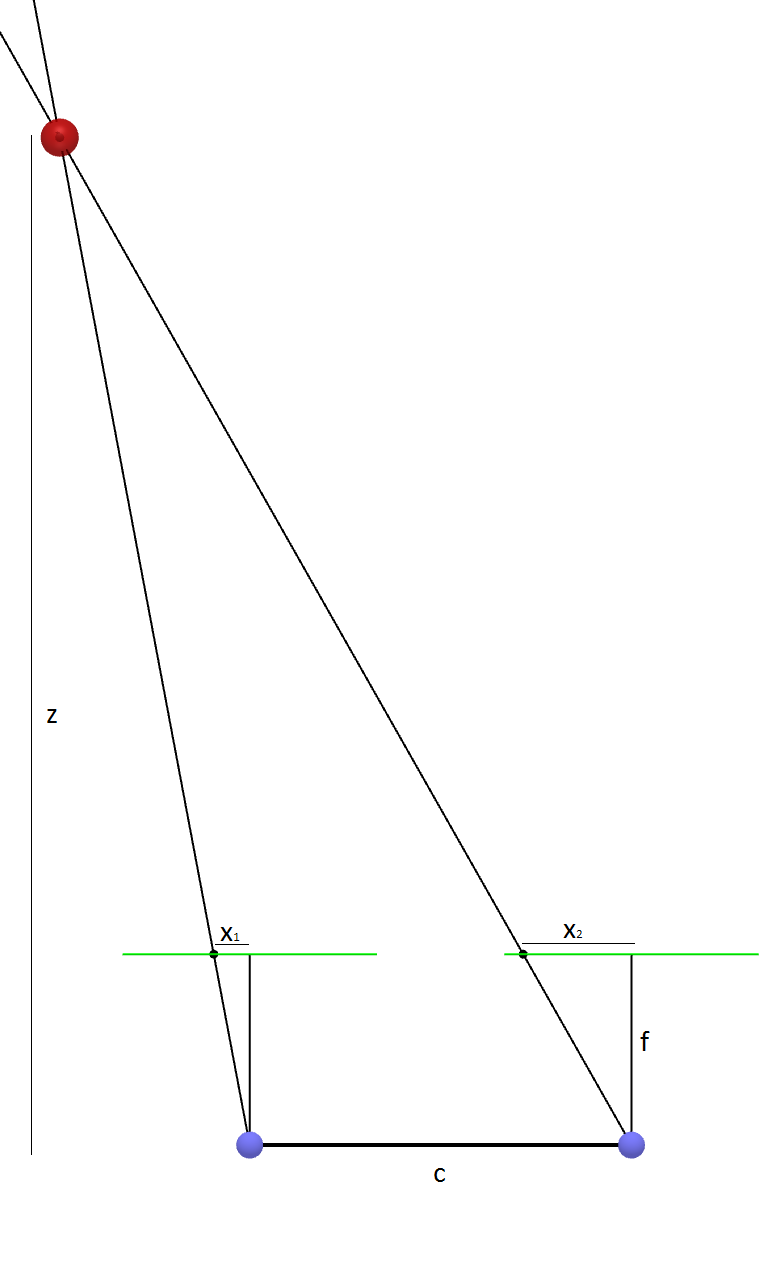
\includegraphics[scale=0.35]{Afstanden.png}
		\caption*{\(z = \frac{c \cdot f}{x_1 - x_2}\)}
	\end{center}
\end{figure}




\end{document}
